% Тут используется класс, установленный на сервере Papeeria. На случай, если
% текст понадобится редактировать где-то в другом месте, рядом лежит файл matmex-diploma-custom.cls
% который в момент своего создания был идентичен классу, установленному на сервере.
% Для того, чтобы им воспользоваться, замените matmex-diploma на matmex-diploma-custom
% Если вы работаете исключительно в Papeeria то мы настоятельно рекомендуем пользоваться
% классом matmex-diploma, поскольку он будет автоматически обновляться по мере внесения корректив
%

% По умолчанию используется шрифт 14 размера. Если нужен 12-й шрифт, уберите опцию [14pt]
\documentclass[14pt]{matmex-diploma-custom}
\usepackage{amsmath}
\usepackage{amssymb}
\usepackage{listings}
\usepackage{amsfonts}
\usepackage{graphicx}
\usepackage{mathtools}
\usepackage{adjustbox}
\usepackage{stmaryrd}
\usepackage{multirow}
\usepackage[dvipsnames]{xcolor}

\usepackage{algorithm}
\usepackage[noend]{algpseudocode}
\usepackage{amssymb}
\usepackage[russian]{babel}

\lstset{
  basicstyle=\ttfamily,
  mathescape
}
%\documentclass[14pt]{matmex-diploma-custom}

\newcommand{\gsv}[1]{\textcolor{red}{#1$^{\text{gsv}}$}}
\newcommand{\simpleton}[1]{\textcolor{ForestGreen}{#1$^{\text{fix}}$}}

\begin{document}
% Год, город, название университета и факультета предопределены,
% но можно и поменять.
% Если англоязычная титульная страница не нужна, то ее можно просто удалить.
\filltitle{ru}{
    chair              = {Математическое обеспечение и администрирование информационных систем \\
                          Системное программирование},
    title              = {Разработка матричного алгоритма поиска путей с контекстно-свободными ограничениями для RedisGraph},
    % Здесь указывается тип работы. Возможные значения:
    %   coursework - Курсовая работа
    %   diploma - Диплом специалиста
    %   master - Диплом магистра
    %   bachelor - Диплом бакалавра
    type               = {bachelor},
    position           = {студента},
    group              = 444,
    author             = {Терехов Арсений Константинович},
    supervisorPosition = {к.ф.-м.н., доцент кафедры информатики СПбГУ},
    supervisor         = {Григорьев С. В.},
    reviewerPosition   = {к.ф.-м.н., Инженер-программист ООО "ИнтеллиДжей Лабс"},
    reviewer           = {Березун Д. А.},
    % chairHeadPosition  = {д.\,ф.-м.\,н., профессор},
    % chairHead          = {Хунта К.\,Х.},
%   university         = {Санкт-Петербургский Государственный Университет},
%   faculty            = {Математико-механический факультет},
%   city               = {Санкт-Петербург},
%   year               = {2013}
}
\filltitle{en}{
    chair              = {Software and Administration of Information Systems \\
                          Software Engineering},
    title              = {Development of matrix-based context-free path querying algorithm for RedisGraph},
    author             = {Terekhov Arseniy},
    supervisorPosition = {PhD, Assistant Professor},
    supervisor         = {Semyon Grigorev},
    reviewerPosition   = {PhD, Software engineer LCC "IntelliJ Labs"},
    reviewer           = {Daniil Berezun}
    % chairHeadPosition  = {professor},
    % chairHead          = {Christobal Junta},
}

\maketitle

\tableofcontents
% У введения нет номера главы
\section*{Введение}
Поиск путей в графе с ограничением в виде формальных языков~\cite{FLCpathProblem} --- это задача, в которой формальные языки используются для задания множества искомых путей. В таком подходе каждый путь соответствует слову, состоящему из меток его рёбер, а ограничением на путь является принадлежность соответствующего ему слова некоторому заданному формальному языку.

В качестве класса формальных языков по иерархии Хомского наибольший интерес представляют контекстно-свободные языки. В отличие от регулярных они обладают большей выразительностью. Поэтому в задаче поиска путей контекстно-свободные ограничения позволяют задавать более сложные отношения между вершинами. Так, например, важный класс запросов поиска вершин, лежащих на одном уровне иерархии~\cite{zhlang-2016}, задаётся только контекстно-свободными, но не регулярными ограничениями. Запросы такого вида, как и другие запросы с контекстно-свободными ограничениями имеют широкое применение в биоинформатике~\cite{bio-application} и при обработке rdf-файлов~\cite{zhlang-2016}.

Наиболее удобным и подходящим инструментом для работы с граф\-структурированными данными являются графовые базы данных. Так же как и реляционные, графовые базы данных поддерживают свой язык запросов. С его помощью графовые базы данных позволяют решать вышеупомянутую задачу поиска путей. Но ограничения на пути, которые поддерживается в наиболее распространённых базах данных, являются в лучшем случае регулярными.

Отсутствие поддержки контекстно-свободных ограничений в графовых базах данных, во-первых, сильно ограничивает выразительность языка запросов. Во-вторых, при необходимости в более сложных запросах разработчикам приходится самим писать алгоритмы, решающие задачу контекстно-свободной достижимости для их частного случая. Так, например, Хуэй Мяо и др.~\cite{datascince-lifecycle} разработали систему хранения и отслеживания версий артефактов, возникающих при научных работах. Вся информация про артефакты хранилась в графовой базе данных. При этом при разработке возникла потребность в выполнении запросов с контекстно-свободными ограничениями для выявления взаимоотношений между различными версиями различных артефактов. Это и послужило началом статьи~\cite{datascince-lifecycle}, в которой приводятся алгоритмы решения частных запросов.

В недавнем исследовании Йохем Куйперс и др.~\cite{Kuijpers:2019:ESC:3335783.3335791} произвели сравнительный анализ наиболее известных алгоритмов поиска путей с конте\-кстно-свободными ограничениями. Алгоритмы запускались на графах, находящихся в хранилище графовой базы данных Neo4j. По результатам исследования было показано, что в контексте Neo4j алгоритмы обладают большим временем работы, и поэтому дальнейшая работа по расширению языка запросов прекратилась. При этом Рустам Азимов~\cite{Azimov:2018:CPQ:3210259.3210264} предоставил матричный алгоритм и его реализацию, которая работает за разумное время на реальных данных. Но, так как алгоритм был реализован вне контекста базы данных, его результат приняли недостаточно показательным. Поэтому вопрос о реализуемости запросов с контекстно-свободными ограничениями в графовых базах данных, а соответственно и о возможности расширения языка запросов для их поддержки остаётся открытым.

\section{Постановка задачи}
Целью данной работы является полная поддержка запросов с конте\-кстно-свободными ограничениями для графовой базы данных. А именно, необходимо предоставить пользователю возможность формулировать запросы с контекстно-свободными ограничениями в терминах одного из существующих стандартных языков запросов и исполнять их в графовой базе данных за приемлемое время. Для достижения этой цели были поставлены следующие задачи.

\begin{itemize}
    \item Выполнить обзор существующих реализаций поддержки запросов с контекстно-свободными ограничениями в графовых базах данных. В результате обзора необходимо выбрать наиболее перспективный с точки зрения производительности алгоритм решения задачи контекстно-свободной достижимости и подходящую для его интеграции базу данных. При выборе базы данных необходимо учитывать как возможность интеграции выбранного алгоритма, так и возможность поддержки одного из стандартных языков запросов, позволяющего выражать контекстно-свободные ограничения.
    \item Интегрировать выбранный на предыдущем шаге алгоритм в выбранную графовую базу данных.
    \item Расширить язык запросов выбранной базы данных конструкциями, необходимыми для выражения контекстно-свободных ограничений.
    \item Произвести замеры производительности полученного решения и сравнить его с существующими решениями.
\end{itemize}


\section{Обзор}

\subsection{Терминология}
Контекстно-свободной грамматикой называется $G = (\Sigma, N, P, S)$, где $\Sigma$ --- алфавит терминальных символов, $N$ --- алфавит нетерминальных символов, $P$ --- множество правил вида $A \rightarrow \alpha$, где $A \in N$, $\alpha \in (\Sigma \cup N)^*$, а $S \in N$ --- выделенный стартовый нетерминал.

% \gsv{про S забыли}.

Языком $L$ над алфавитом $\Sigma$ называется любое подмножество $2^{\Sigma^*}$. Языком, порождаемой грамматикой G, является множество $L(G) = \{S \xRightarrow{*} \beta, \beta \in \Sigma^*\}$, где $S \xRightarrow{*} \beta$ означает, что из нетереминала $S$ путём последовательного применения правил грамматики выводится $\beta$.

Контекстно-свободная грамматика $G = (\Sigma, N, P, S)$ находится в осла\-бленной нормальной форме Хомского, если любое её правило имеет вид $A \rightarrow BC$, где $A, B, C \in N$, либо $A \rightarrow a$, где $A \in N, a \in \Sigma$. В отличие от нормальной формы Хомского в ослабленной, во-первых, допускается присутствие стартового нетерминала $S$ в правых частях правил грамматики, во-вторых, запрещаются правила вида $S \rightarrow \epsilon$, где $\epsilon$ --- пустая строка.

% \gsv{Это не нормальная форма Хомского. У НФХ есть дополнительные ограничения. Мы называем то, что здесь, ослабленной НФХ. Важно отдельно проговорить разницу с НФХ.}

В задаче поиска путей с ограничениями в виде формальных языков дан граф $(V, E)$, разметка его рёбер $l: E \rightarrow \Sigma$ и язык $L$ над алфавитом $\Sigma$. Требуется найти множество всех пар вершин, между которыми существует путь, метки на рёбрах которого образуют слово в заданном языке. То есть требуется найти следующее множество:
\[\{(v, to): \exists p=(e_1,...,e_n) \in E^*: l(e_1)...l(e_n) \in L,~src(e_1)=v,~dst(e_n)=to\}\]
Здесь $src(e)$ и $dst(e)$ для $e \in E$ означают начальную и конечную вершину ребра $e$. В данном контексте язык $L$ называется языком ограничений.
% \gsv{У Вас вершины v и to никак с путём не связаны}

Задача поиска путей с контекстно-свободными ограничениями --- это задача поиска путей в виде формальных языков, в которой язык задаётся контекстно-свободной грамматикой.

\subsection{Графовые базы данных}
Графовые СУБД\footnote{СУБД --- Система управления базами данных} (далее просто графовые базы данных) --- это разновидность СУБД, в которой данные хранятся в виде графов. В отличие от других разновидностей, в графовых базах данных отношения между объектами так же важны, как и сами объекты.

Основной моделью представления графов в таких базах данных является gpraph property model~\cite{graph-propery-model}. В ней каждая сущность может содержать набор свойств в формате ключ-значение. Основными сущностями являются узлы и отношения. Узлы соответствуют вершинам графа и помимо свойств могут иметь несколько меток. Отношения соответствуют рёбрам и имеют ровно одну метку, которая называется типом отношения. На рисунке~\ref{fig:graph_bd_1} показан небольшой пример графа в такой модели. 

\begin{figure}[h]
\centering
    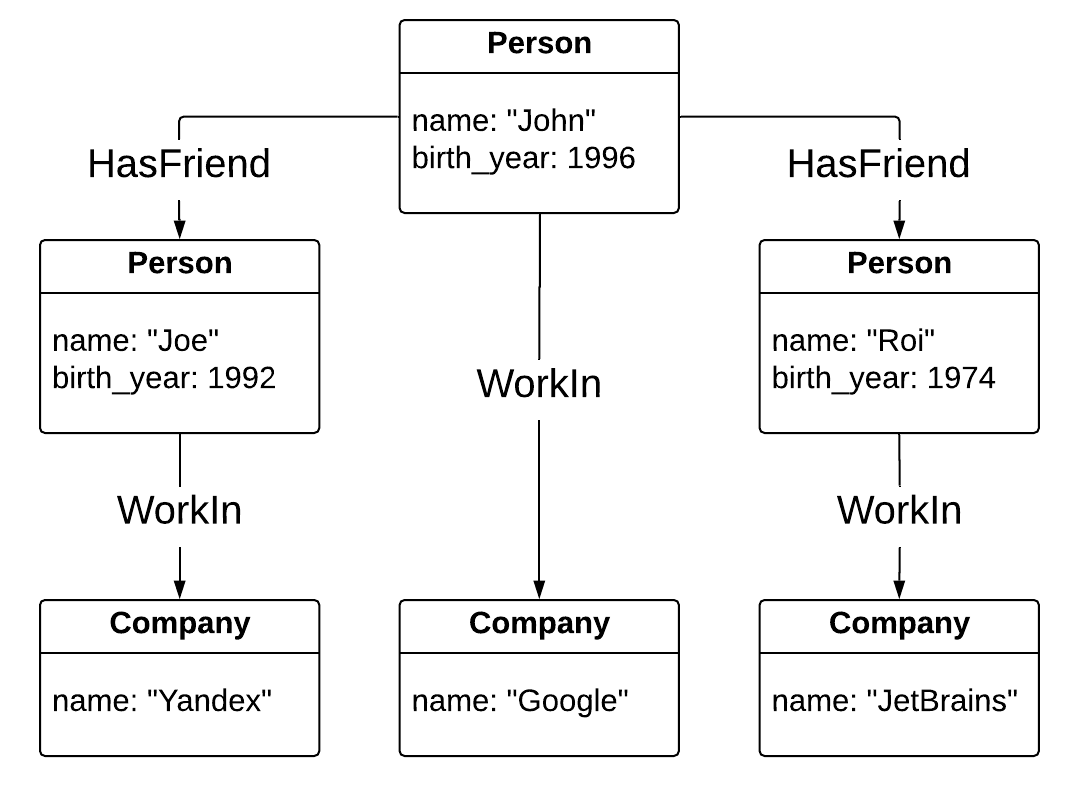
\includegraphics[width=0.7\linewidth]{pictures/graph_bd_1.png}
    \caption{Пример социального графа}
    \label{fig:graph_bd_1}
\end{figure}

Для работы с графами графовые базы данных предоставляют язык запросов, самым популярным из которых является Cypher~\cite{cypher-language}. В нём главный интерес представляют запросы вида сопоставления с образцом. Они позволяют задавать интересующие пути или подграфы в виде шаблонов и описывать информацию, которую нужно извлечь после удачного сопоставления. На рисунке~\ref{code:cypher_query} приведён пример такого запроса. Шаблон пути описывается в выражении MATCH. В нём между круглыми скобками задаются шаблоны вершин, а между квадратными шаблоны рёбер. Таким образом в данном примере задаются следующие ограничения: путь должен начинаться из вершины с меткой Person и именем John и состоять из двух рёбер, первое из которых должно иметь тип HasFriend, а второе WorkIn. В выражении RETURN задаётся информация, которую нужно извлечь. В данном примере это имя последней в пути вершины. В итоге ответом на такой запрос являются имена компаний, в которых работают друзья Джона. Результатом работы этого запроса на графе из рисунка~\ref{fig:graph_bd_1} является множество \{"Yandex", "JetBrains"\}.

\lstset{
   basicstyle=\fontsize{14}{14}\selectfont\ttfamily
}

\begin{figure}[h]
\begin{lstlisting}[language=sql]
MATCH (p:Person)-[:HasFriend]->()-[:WorkIn]->(to)
WHERE p.name = "John"
RETURN to.name
\end{lstlisting}
\caption{Пример конечного запроса на языке Cypher}
\label{code:cypher_query}
\end{figure}

С формальной точки зрения шаблоны пути в выражении MATCH позволяют поставить задачу поиска путей с ограничениями в виде формальных языков. Так в запросе на рисунке~\ref{code:cypher_query} языком ограничений является конечный язык $\{(HasFriend, WorkIn)\}$. Для запроса на рисунке~\ref{code:cypher_query_2} ограничением является регулярный язык $\{A, B\}^*$. 

\begin{figure}[h]
\begin{lstlisting}[language=sql]
MATCH (v)-[:A | :B *]->(to)
RETURN to.name
\end{lstlisting}
\caption{Пример регулярного запроса на языке Cypher}
\label{code:cypher_query_2}
\end{figure}

При этом регулярные ограничения поддерживаются лишь частично и позволяют искать только пути произвольной длины с заданными метками на рёбрах, а более глубокие регулярные выражения не поддерживаются. Поэтому на текущий момент язык запросов довольно ограничен.

\subsection{Существующие решения}
Как было упомянуто раннее, ни одна графовая база данных не поддерживает запросов с контекстно-свободными ограничениями. Тем не менее существуют альтернативные решения поддержки таких запросов. 

\subsubsection{Парсер-комбинаторы для Neo4j}\label{sec:pareser-combinators}
В 2018 году группой исследователей из JetBrains Research на основе библиотеки Meerkat была разработана библиотека для поддержки запросов с контекстно-свободными ограничениями~\cite{parser-combinators}. Она использует графовую базу данных Neo4j~\cite{neo4j} как хранилище графов и позволяет задавать запросы в виде парсер-комбинаторов. Основным достоинством данной работы является то, что с помощью этой библиотеки кроме контекстно-свободных запросов можно выразить базовую часть языка Cypher. Но так как конкурировать с оригинальной реализацией выполнения запросов Neo4j очень сложно, это достигается вместе c сильной потерей производительности. Кроме этого контекстно-свободные запросы обрабатываются также достаточно медленно.

Таким образом данное решение является альтернативой языка запросов Neo4j, а не его расширением. Из-за медленного времени работы такое решение подходит только для работы с небольшими графами. 

\subsubsection{Расширение языка запросов SPARQL}\label{subsection:cypher-extention-2}
%Про sparql%
В 2016 Сяованг Чжан предоставил язык cfSPARQL~\cite{zhlang-2016} --- расширение языка SPARQL, который способен выразить запросы с контекстно-свободными ограничениями. Также он привёл алгоритм для вычисления таких запросов и замеры производительности. Но, во-первых, работа была сделана вне контекста графовой базы данных, а во-вторых, время работы предложенного алгоритма было больше, чем время работы парсер-комбинаторов.

\subsubsection{Существующие реализации алгоритмов решения задачи контекстно-свободной достижимости}
Основной сложностью расширения языка запросов для поддержки запросов с контекстно-свободными ограничениями является долгое время работы соответствующих алгоритмов. Так, например, в 2019 году Йохем Куйперс и другие исследователи с целью попытки расширения языка запросов Cypher для графовой базы данных Neo4j произвели сравнительный анализ производительности наиболее известных алгоритмов решения задачи контекстно-свободной достижимости.

В данном исследовании были рассмотрены и произведены замеры времени работы алгоритма Элле Хелингса~\cite{hellings-2015}, основанного на атрибутных грамматиках, восходящего алгоритма Фреда Сантоса~\cite{santos-2018}, матричного алгоритма Рустама Азимова~\cite{Azimov:2018:CPQ:3210259.3210264} и алгоритма Петтери Севона~\cite{bio-application}. Все алгоритмы были интегрированы в Neo4j и запускались на графах, находящихся в её хранилище. Алгоритмы были написаны на языке Java, при этом их реализация являлась однопоточной.

% \gsv{В таких местах надо сразу ссылку на алгоритм давать.}

По результатам замеров производительности было показано, что время работы алгоритмов является слишком большим и неприемлемым для широкого практического использования. Поэтому дальнейшая работа по интеграции и расширению языка запросов была приостановлена.

Тем не менее, матричный алгоритм Рустама Азимова в сравнительном анализе Йохема Куйперса был реализован без необходимых матричных библиотек, которые могут сильно уменьшить время его работы. Так, например, в исследовании Никиты Мишина и др.~\cite{azimov-evalution} был произведён сравнительный анализ времени работы нескольких реализаций алгоритма Рустама Азимова, основанных на различных специализированных матричных библиотеках. Графы и запросы к ним были взяты из объемлющего набора данных CFPQ\_Data~\cite{cfpq-data}, предоставленного лабораторией языковых инструментов JetBrains Research. 

Результаты замеров Никиты Мишина и др. показали, что при грамотной реализации алгоритма Рустама Азимова и использовании подходящих матричных библиотек можно добиться очень высокой производительности. Поэтому, так как основной проблемой применимости запросов с контекстно-свободными ограничениями является долгое время работы соответствующих алгоритмов, в качестве алгоритма решения задачи конте\-кстно-свободной достижимости был выбран матричный алгоритм Рустама Азимова.

\subsection{Матричный алгоритм Рустама Азимова}\label{sec:matrix-algo}
Выбранный в предыдущей главе алгоритм Рустама Азимова~\cite{Azimov:2018:CPQ:3210259.3210264}, в отличие от других алгоритмов решения задачи контекстно-свободной достижимости~\cite{hellings-2015, santos-2018, zhlang-2016}, работает с графами в виде разреженных матриц смежности. Данный алгоритм состоит из последовательности операций над разреженными матрицами, время работы которых зависит не от размеров матричных операндов, а от количества их ненулевых элементов.

На вход алгоритму (см. алгоритм 1) поступает помеченный граф $D=(V,E)$ и контекстно-свободная грамматика $G=(\Sigma, N, P, S)$ в ослабленной нормальной форме Хомского. Для каждого нетерминала $A$ в ассоциативном массиве $T$ хранится соответствующая ему булева матрица $T[A]$. На всём этапе алгоритма поддерживается следующий инвариант: $T[A]_{i,j} = 1$ равносильно существует пути, метки на рёбрах которого образуют слово, выводящееся из нетерминала $A$. На первом этапе происходит инициализация матриц с помощью простых правил грамматики, после чего инвариант выполняется для всех путей единичной длины. На втором этапе происходит транзитивное замыкание, после чего этот инвариант верен для всех путей. Результатом данного алгоритма является матрица, соответствующая стартовому нетерминалу $S$.

%  Это позволяет для его реализации использовать многопоточные матричные библиотеки, с помощью которых можно добиться очень высокой производительности. Поэтому на текущий момент алгоритм Рустама Азимова показывает наилучшее время работы на практике.

\begin{algorithm}
\caption{Матричный алгоритм Рустама Азимова}

\begin{algorithmic}[1]
\Function{contextFreePathQuerying}{$D$, $G$}
    \State{$n =$ getNodeCount(D)}
    \State{$N =$ getAllNonterms(G)}
    \State{$E =$ getEdges($D$)}
    \State{$P =$ getRules($G$)}
    \State{$S =$ getStartNonterm($G$)}
    \State{$T = \{A \rightarrow \varnothing_{n \times n} : A \in$ $N$ \} }
    \ForAll{$(v, to, label) \in E$}
    \Comment{Инициализация матриц}
        \ForAll{$A \rightarrow label \in P$}
            \State{$T[A]_{i,j} = 1$}
        \EndFor
    \EndFor    
    \While{$\exists A: T[A]$ is changing}
    \Comment{Вычисление замыкания}
        \ForAll{$A \rightarrow BC \in P$}
            \State{$T[A] \oplus= T[B] \otimes T[C]$}
        \EndFor
    \EndWhile
\State \Return $T[S]$
\EndFunction

\end{algorithmic}
\end{algorithm}

Практическое время работы алгоритма Рустама Азимова сильно зависит от производительности используемой матричной библиотеки. Это накладывает некоторые ограничения на выбор подходящей графовой базы данных, так же как и возможность представления графов в матричном виде.

\subsection{RedisGraph}
RedisGraph~\cite{redis-graph} --- это высокопроизводительная графовая база данных, поддерживающая язык запросов Cypher. В отличие от наиболее распространённой графовой базы данных Neo4j~\cite{neo4j}, RedisGraph написан на языке Си и для работы с данными использует Redis~\cite{redis}, основным достоинством которого является возможность хранить данные прямо в оперативной памяти. Это позволяет RedisGraph быстро обрабатывать пользовательские запросы.

Также RedisGraph является единственной графовой базой данных, которая работает с графами в виде разреженных матриц смежности и транслирует запросы языка Cypher в матричные выражения. Для представления графов в таком виде и работы с ними в терминах линейной алгебры используется мощный матричный фреймворк GraphBlas~\cite{graph-blas}. Его реализация SuiteSparse~\cite{suite-sparse} является многопоточной и сильно оптимизирована, что позволяет RedisGraph добиться высокой производительности.

Из всего этого следует, что RedisGraph идеально подходит для интеграции матричного алгоритма. Во-первых, графы представляются в необходимом алгоритму виде, что позволит избежать издержек на конвертацию форматов. Во-вторых, использование SuiteSparse для вычисления матричных операций позволит добиться высокой производительности. Поэтому RedisGraph был выбран в качестве графовой базы данных для интеграции матричного алгоритма и расширения языка запросов.

% Так как алгоритм Рустама Азимова работает с матричным представлением графа,, как наиболее подходящий для интеграции матричного алгоритма.

\subsection{Расширение языка Cypher}\label{subsection:cypher-extention}
На текущий момент оригинальная версия языка Cypher, используемая в том числе и в RedisGraph, не поддерживает запросов с контекстно-свободными ограничениями. Но тем не менее в 2017 году был разработан черновой вариант спецификации расширения Cypher~\cite{cypher-specification}, которая вводит в язык шаблоны путей. Они позволяют выразить более сложные запросы, в том числе запросы с контекстно-свободными ограничениями.

Шаблоны путей являются альтернативой шаблонам рёбер, которые есть в оригинальном Cypher. Они, как и шаблоны рёбер, могут встречаться в выражении MATCH и иметь своё направление. Кроме этого в глобальной области запроса им можно задавать имя, на которое потом можно ссылаться внутри других шаблонов.

Шаблон пути представляет из себя регулярное выражение над некоторыми примитивами. В качестве таких примитивов могут выступать шаблоны рёбер, шаблоны вершин и ссылки на именованные шаблоны путей. Также любым подвыражениям можно задавать своё направление. Основная часть конкретного синтаксиса данного расширения приведена на рисунке~\ref{fig:cypher_syntax}.

\begin{figure}[]
\begin{align*}
\begin{split}
PathPattern     &= ["<"],~"-/",~PathExpression,~"/-",~[">"]\\
PathExpression  &= \{PathAlternative\}\\
PathAlternative &= PathRepetition,~\{"|", PathRepetition\}\\
PathRepetition  &= ["<"],~PathBase,~[">"],~("*")
\end{split}\\
\begin{split}
PathBase &= PathEdge \\
         &~~|~PathNode \\
         &~~|~PathReference \\
         &~~|~"[",~PathExpression,~"]"
\end{split}\\
\begin{split}
PathEdge      &= Label \\
PathNode      &= "(",~[Label,~\{"|",~Label\}],~")" \\
PathReference &= "\sim",~SymbolicName; \\
Label         &= ":",~LabelName
\end{split}
\end{align*}
\caption{Расширение конкретного синтаксиса Cypher}
\label{fig:cypher_syntax}
\end{figure}

Каждый шаблон пути задаёт отношение на множестве вершин. Поэтому семантикой языка шаблонов путей $L_{P}$ в контексте графа $G(V, E)$ является отображение $\llbracket \cdot \rrbracket_{G}: L_P \rightarrow V \times V$, которое каждому шаблону $p\in L_P$ сопоставляет множество пар вершин, между которыми существует путь, удовлетворяющий данному шаблону $p$. 

Подробное описание данной семантики приводится в таблице~\ref{tab:cypher_sematic}.  В ней наибольший интерес представляют именованные шаблоны путей, так как именно с помощью них можно выразить запросы с контекстно-свободными ограничениями. Все именованные шаблоны путей $S_i = p_j$ можно рассматривать как правила контекстно свободной грамматики с алфавитом нетерминалов $\{S_i\}_{i=1}^n$. Тогда каждый нетерминал $S_j$ порождает язык $L_{S_j} \subset L_p$, а семантикой соответствующего именованного шаблона пути $S_j=p_j$ является множество $\bigcup\limits_{p \in L_{s_j}} \llbracket p \rrbracket_{G}$.

На рисунке~\ref{code:cypher_query_3} приведён пример запроса в расширенном синтаксисе. В нём декларируется именованный шаблон S, который задаёт множество правильных скобочных последовательностей над ребрами с типом L и R. Далее в выражении MATCH задаётся шаблон пути, состоящий из ссылки на шаблон S. Таким образом результатом обработки запроса является множество всех пар вершин, между которыми существует путь, метки на рёбрах которого образуют правильную скобочную последовательность. 

\begin{table}[h!]
\begin{adjustbox}{max width=\textwidth}
\begin{tabular}{|c|c|c|}
\hline
$p \in L_P$                                                                                  & $\llbracket p \rrbracket_{G}$                                                                                                                                                                                   & Описание шаблона пути                                                                                                         \\ \hline
\hline
()                                                                                            & $\{(v, v): v \in V\}$                                                                                                                                                                                           & \begin{tabular}[c]{@{}c@{}}Пустой путь, состоящий из \\ одной произвольной вершины\end{tabular}                               \\ \hline
:a                                                                                            & $\{e=(v,to): e \in E, type(e)=a\}$                                                                                                                                                                              & \begin{tabular}[c]{@{}c@{}}Путь единичной длины,\\  состоящий из ребра с типом $a$\end{tabular}                               \\ \hline
(:b)                                                                                          & $\{(v, v): v \in V, label(v)=b\}$                                                                                                                                                                               & \begin{tabular}[c]{@{}c@{}}Пустой путь, состоящий из одной\\  вершины, помеченной меткой $b$\end{tabular}                     \\ \hline
$\alpha~\beta$                                                                                & $\llbracket \alpha \rrbracket_{G}\circ \llbracket \beta \rrbracket_{G}$                                                                                                                                         & Конкатенация путей $\alpha$ и $\beta$                                                                                         \\ \hline
$\alpha~|~\beta$                                                                              & $\llbracket \alpha \rrbracket_{G}\cup \llbracket \beta \rrbracket_{G}$                                                                                                                                          & Альтренатива между путями $\alpha$ и $\beta$                                                                                  \\ \hline
$[\alpha]$                                                                                    & $\llbracket \alpha \rrbracket_{G}$                                                                                                                                                                              & \begin{tabular}[c]{@{}c@{}}Квадратные скобки позволяют \\ группировать  выражения \\ для задания ассоциативности\end{tabular} \\ \hline
\textless{}$\alpha$                                                                           & $\{(to, v): (v, to) \in \llbracket \alpha \rrbracket_{G}\}$                                                                                                                                                     & Путь, обратный к пути $\alpha$                                                                                                \\ \hline
\textless{}$\alpha$\textgreater{}                                                             & $\llbracket \alpha~|~$\textless{}$\alpha \rrbracket_{G} $                                                                                                                                                       & \begin{tabular}[c]{@{}c@{}}Альтернатива между путём $\alpha$ и\\ обратным к нему\end{tabular}                                 \\ \hline
$\alpha^*$                                                                                    & $\llbracket \alpha \rrbracket_{G}^{*}$                                                                                                                                                                          & \begin{tabular}[c]{@{}c@{}}Путь, состоящий из\\ конкатенации 0 или более путей $\alpha$\end{tabular}                          \\ \hline
\begin{tabular}[c]{@{}c@{}}$\{S_i = p_i\}_{i=1}^{n}$\\ -- named\\  path patterns\end{tabular} & \begin{tabular}[c]{@{}c@{}}$P = \{S_i \rightarrow p_i\}_{i=1}^n$\\ $Gram_j = (\Sigma, \{S_i\}_{i=1}^n, P, S_j)$\\ $\llbracket S_j \rrbracket_{G} = \bigcup\limits_{p \in L(G)}{\llbracket p \rrbracket_{G}}$\end{tabular} & Именнованые шалоны путей                                                                                                      \\ \hline
$\sim$$S$                                                                                     & $\llbracket S \rrbracket_{G}$                                                                                                                                                                                   & \begin{tabular}[c]{@{}c@{}}Ссылка на именнованный\\  шаблон пути\end{tabular}                                                 \\ \hline
\end{tabular}
\end{adjustbox}
\caption{Семантика языка шаблонов путей}
\label{tab:cypher_sematic}
\end{table}

\begin{figure}[h!]
\begin{lstlisting}[language=sql]
PATH PATTERN S = ()-/ [:L ~S :R] | [~S ~S] | () /-()
MATCH (v)-/ ~S /-(to)
RETURN v, to
\end{lstlisting}
\caption{Пример запроса в расширенном синтаксисе Cypher}
\label{code:cypher_query_3}
\end{figure}

Данная спецификация расширения Cypher была представлена официальными разработчиками и сильно расширяет выразительность языка, предоставляя удобную возможность выражать запросы как с регулярными, так и с контекстно-свободными ограничениями. Поэтому в моей работе приводится поддержка выполнения запросов именно для этого расширения языка.

% \gsv{Не хватает какого-то чёткого вывода про то, что вот именно это мы и буем использовать.}

\section{Реализация}
По результатам обзора было решено реализовать поддержку расширения языка Cypher, представленную в главе~\ref{subsection:cypher-extention}, для графовой базы данных RedisGraph. За основу алгоритма, решающего задачу поиска путей с контекстно-свободными ограничениями, был взят матричный алгоритм Рустама Азимова, описанный в главе~\ref{sec:matrix-algo}.

% \gsv{И зжесь надо ещё раз подитожить в духе "по результатм обзора было решено сделать то и это с использованием того и сего"}

\subsection{План выполнения запроса}\label{execution-plan}
В RedisGraph основной частью обработки запроса является построение плана его выполнения. Её часть, которая относится к шаблонам путей приведена на рисунке~\ref{fig:execution_plan}. В ней зелёным цветом выделено то, что было добавлено или расширено.

В самом начале, после получения запроса строится его абстрактное синтаксическое дерево \textit{AST}. Далее, из него извлекаются именованные и неименованные шаблоны путей \textit{PathPattern} и \textit{NamedPathPatterns}, после чего они преобразуются в более удобное промежуточное представление \textit{PathExpr}. При этом, для дальнейшего связывания ссылок, именованные шаблоны сохраняются в глобальном контексте запроса \textit{PathPatternCtx}.

На следующем этапе происходит трансляция промежуточных представлений \textit{PathExpr} в матричные выражения \textit{AlgebraicExpression}. В них операндами являются либо матрицы, полученные из указанного в запросе графа \textit{GraphCtx}, либо ссылки на именованные шаблоны путей из \textit{PathPatternCtx}. Основной идеей трансляции является то, что после вычисления матричного выражения получается матрица, которая задаёт то же самое отношение на множестве вершин, что и исходный шаблон пути.

Далее каждое такое выражение формирует новую операцию плана выполнения запроса \textit{CfpqTraverseOp}. При её вычислении сначала происходит запуск расширенной версии матричного алгоритма Рустама Азимова. Он решает задачу контекстно-свободной достижимости, заданной именованными шаблонами путей. После этого все ссылки в матричном выражении заменяются на полученные в ходе алгоритма матрицы и происходит вычисление матричного выражения. Каждая такая операция добавляется в план выполнения запроса.

%  \gsv{Используйте \textit{CfpqTraverseOp} вместо долларов для длинных слов. Они тогда не распадаются из-а лишних пробелов.}

\begin{figure}[H]
\centering
    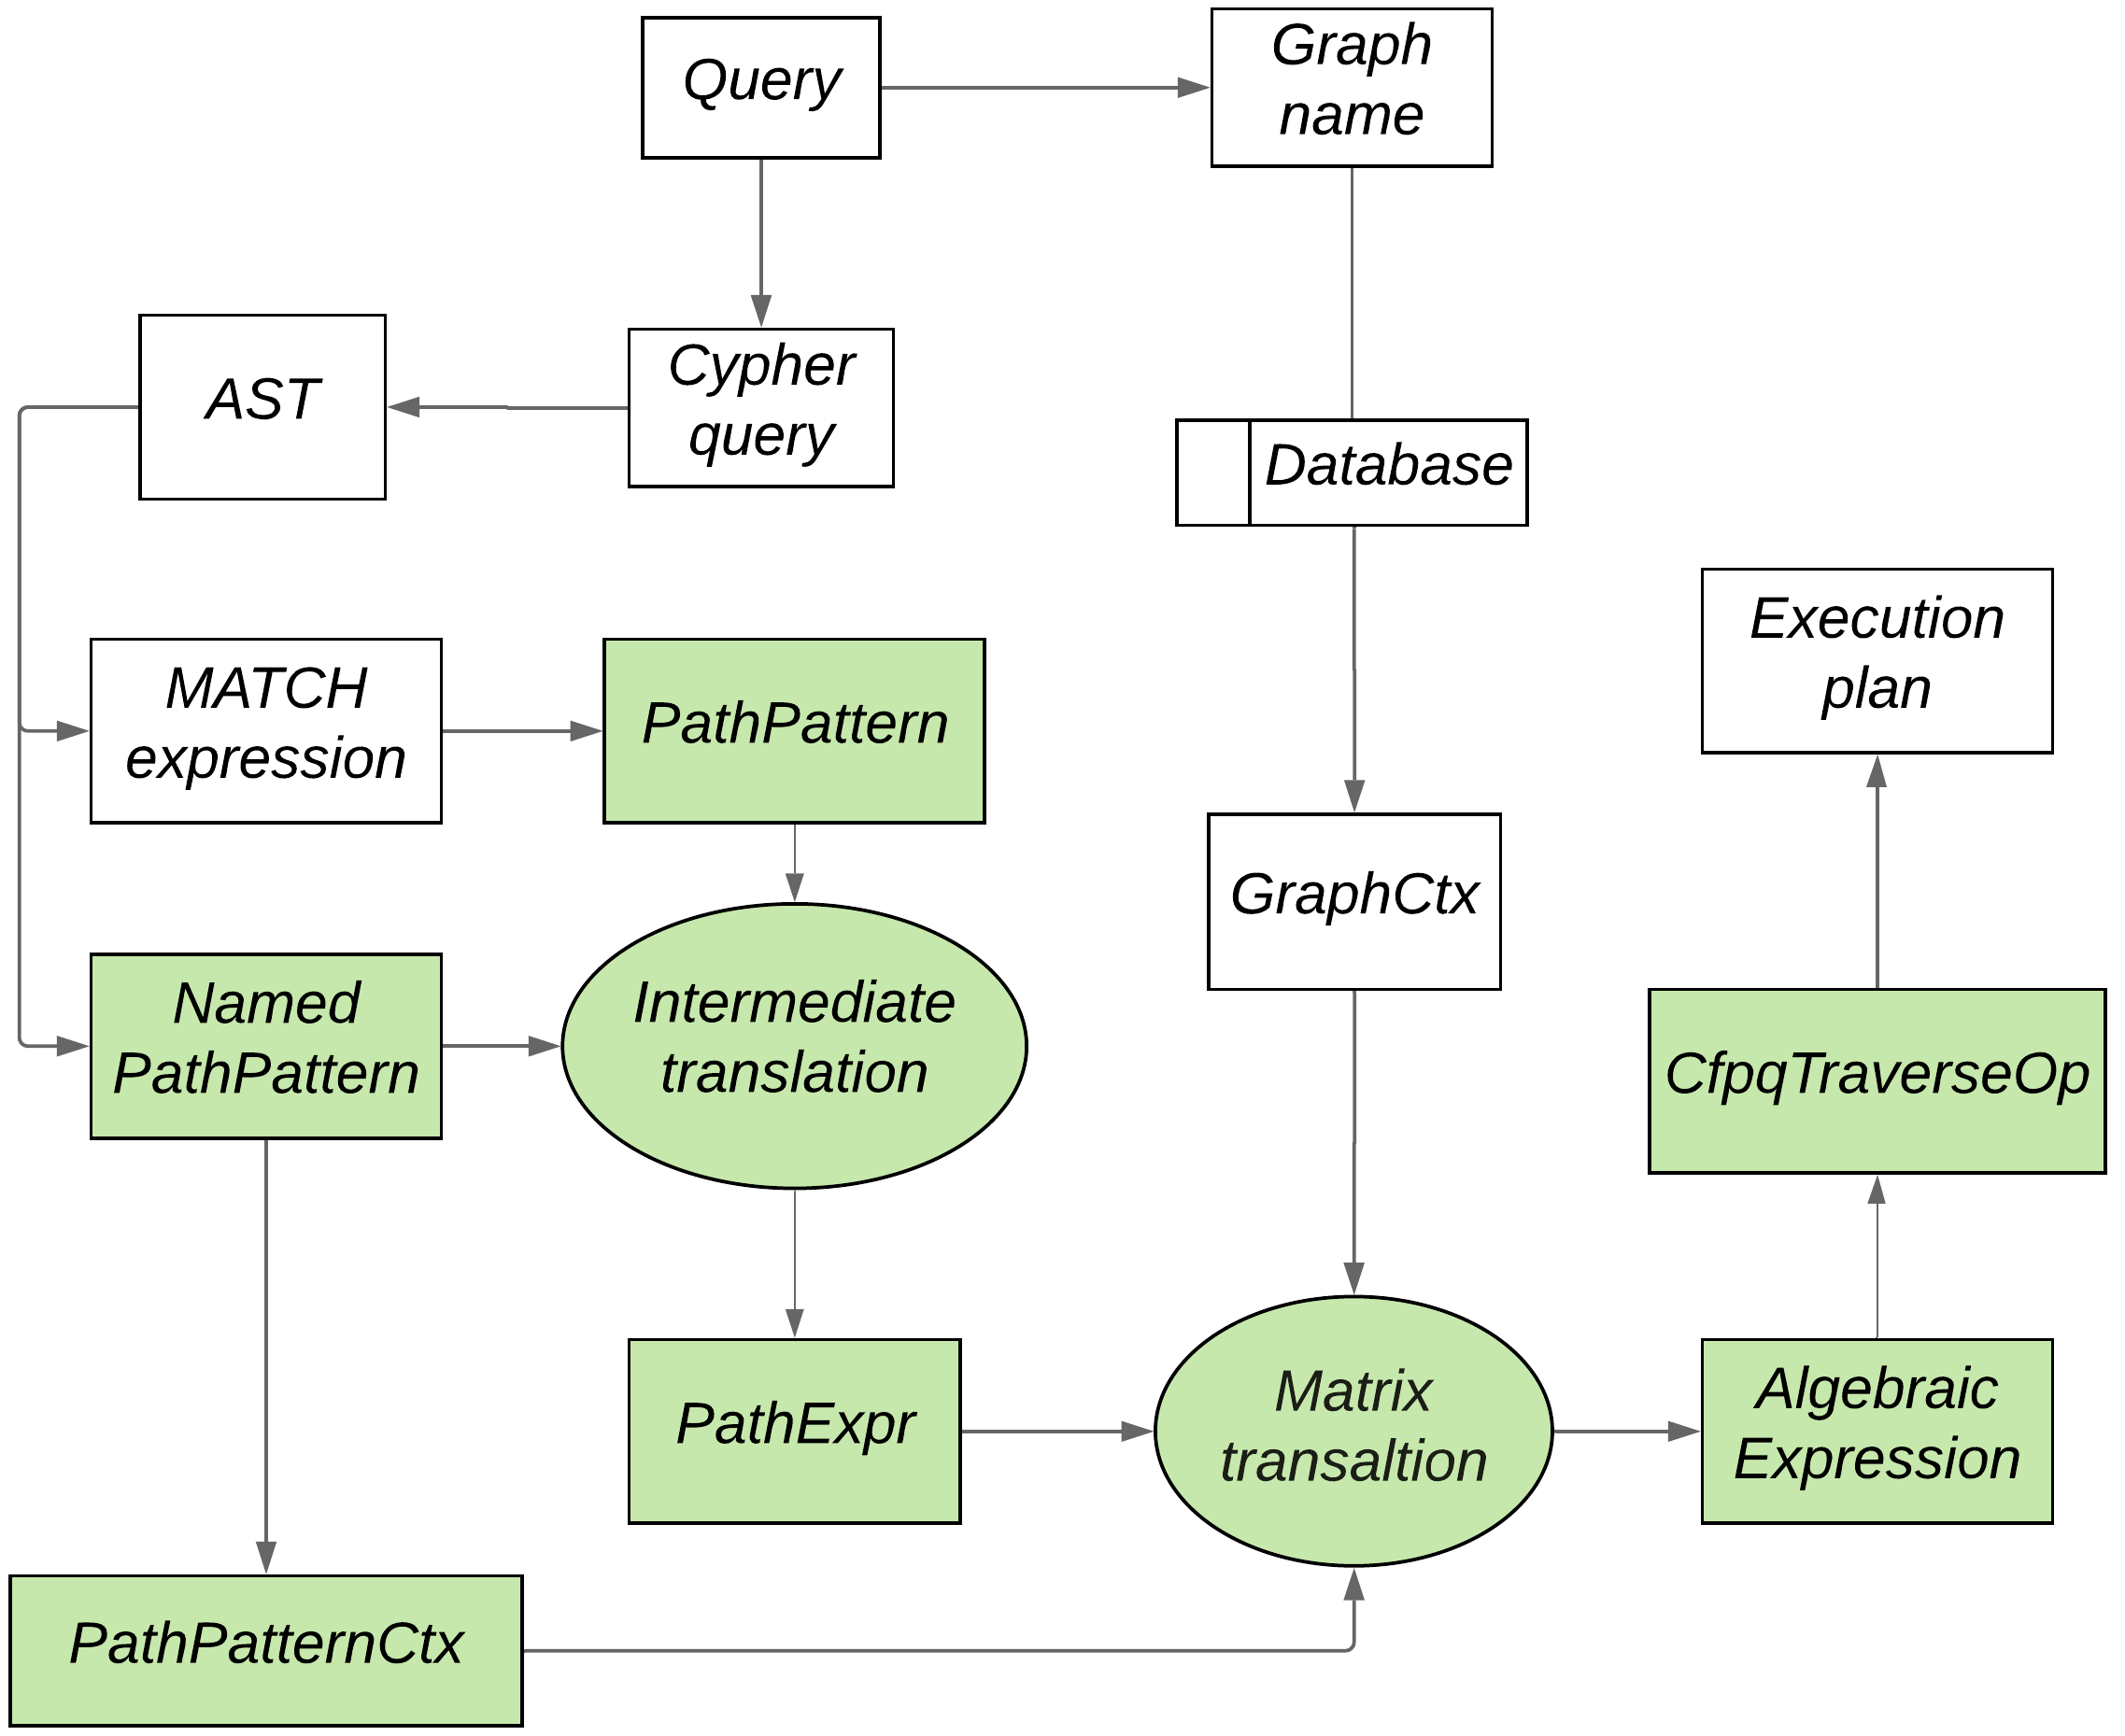
\includegraphics[width=1.0\linewidth]{pictures/execution_plan_3.png}
    \caption{Расширение построения плана выполнения запроса}
    \label{fig:execution_plan}
\end{figure}

\subsection{Промежуточное представление}\label{matrix-translation}
Шаблоны путей, полученные из \textit{AST}, транслируются в промежуточное представление \textit{PathExpr}. Оно позволяет задавать более простой абстрактный синтаксис, который описан на рисунке~\ref{fig:intermidiate_repr}. 

Таким образом, альтернативе и конкатенации шаблонов соответствуют \textit{PathAlt} и \textit{PathSeq}, \textit{PathGroup} позволяет задавать направление пути и наличие замыкания, а \textit{PathBasic} соответствует либо примитивным шаблонам \textit{PathNode}, \textit{PathEdge} и \textit{PathRef}, либо целому выражению \textit{PathExpr}. Примеры промежуточного представления шаблонов приведены в таблице~\ref{tab:inter_examples}.
\begin{figure}[h!]
\begin{align*}
\begin{split}
PathExpr=~ &PathSeq(PathExpr,~PathExpr)~|\\
           &PathAlt(PathExpr,~PathExpr)~|\\
           &PathGroup(PathBasic, direction, range)
\end{split}\\
\begin{split}
PathBasic=~ &PathNode(label)~|\\
            &PathEdge(type)~~|\\
            &PathRef(name) ~~|\\
            &PathExpr
\end{split}\\
\begin{split}
direction \in ~&\{inbound,~outbound,~bidirectional\}\\
range \in     ~&\{*, \varnothing\}
\end{split}
\end{align*}
\caption{Промежуточное представление PathExpr}
\label{fig:intermidiate_repr}
\end{figure}

\begin{table}[h]
\centering
\begin{adjustbox}{max width=\textwidth}
\begin{tabular}{|c|l|}
\hline
$L_p$                        & \multicolumn{1}{c|}{PathExpr}                                                                                                        \\ \hline
{[}:A :B{]} | (:C)           & \begin{tabular}[c]{@{}l@{}}$PathAlt($\\ $~~~~PathSeq(PathEdge("A"),~PathEdge("B"))$\\ $~~~~PathNode("C")$\\ $)$\end{tabular}         \\ \hline
\textless{}{[}:A $\sim$S{]}* & \begin{tabular}[c]{@{}l@{}}$PathGroup($\\ $~~~~PathSeq(PathEdge("A"),~PathRef("S")),$\\ $~~~~inbound,$\\ $~~~~*,$\\ $)$\end{tabular} \\ \hline
\end{tabular}
\end{adjustbox}
\caption{Примеры промежуточного представления запросов}
\label{tab:inter_examples}
\end{table}

\newpage
\subsection{Трансляция в матричные выражения}
Как было упомянуто ранее, RedisGraph представляет графы в виде разреженных матриц. А именно каждый граф $G$ задаётся следующей тройкой $(A \in M_{n\times n},~lab \in Labels \rightarrow Diag_n,~rel \in RelTypes \rightarrow M_{n \times n})_G$. Здесь $M_{n \times n}$ означает полукольцо булевых матриц, а $Diag_n$ полукольцо диагональных булевых матриц. Матрица $A$ служит матрицей смежности графа, а отображения $lab$ и $rel$ сопоставляют меткам вершин и типам рёбер соответствующие булевы матрицы. Таким образом, ребро $(v, to)$ графа $G$ имеет тип $a$ тогда и только тогда, когда $rel(a)_{v,to} = 1$.  Таким же образом, принадлежность метки $l$ вершине $v$ равносильно $lab(l)_{v,v}=1$.

Любую булеву матрицу $M$, участвующую в задании графа $G(V, E)$, можно рассматривать как отношение на множестве вершин $R(M) = \{(v, to):~M_{v,to}=1\}$. Операциями сложения и умножения в булевом полукольце являются дизъюнкция и конъюнкция. Поэтому умножению матриц $A*B$ соответствует композиция отношений $R(A) \circ R(B)$, сложению $A+B$ соответствует объединение отношений $R(A) \cup R(B)$, а транспонированная матрица $A^T$ соответствует обратному к R(A) отношению $R(A)^{-1}$. Такая взаимосвязь между матричными операциями и отношениями лежит в основе алгоритма трансляции, приведённом на рисунке~\ref{algo:translation}.

Данный алгоритм является рекурсивным и принимает на вход промежуточное представление шаблона пути $expr$, представление графа $g$ и контекст именованных шаблонов путей $pathCtx$. Целевым языком трансляции является простой язык матричных выражений, приведённый на рисунке~\ref{fig:alg-expr}.

Базовым случаем рекурсии являются примитивные шаблоны \textit{Path\-Node}, \textit{PathEdge} и \textit{PathReference}, которые транслируются в операнды матричного выражения. Для первых двух соответствующие матрицы извлекаются из графа с помощью функций \textit{GetLabel\-Matrix} и \textit{GetRelation\-Matrix}. При этом случай $label = \varnothing$ соответствует шаблону пути, состоящему из одной произвольной вершины. Поэтому такой путь задаётся тождественным отношением $R(I)$, где $I$ --- единичная матрица. Для \textit{Path\-Reference} создаётся ссылка на матрицу именованного шаблона, которая будет вычислена на следующем этапе при выполнении алгоритма контекстно-свободной достижимости.

Трансляция для шаблонов \textit{PathSeq} и \textit{PathAlt} происходит одинаковым образом --- сначала происходит трансляция дочерних шаблонов, а потом из полученного результата образуются операции умножения или сложения. Такая трансляция обосновывается семантикой шаблонов альтернативы и конкатенации, приведенной в главе~\ref{subsection:cypher-extention}, и связью отношений с матричными операциями, описанными раннее.

Наиболее интересным случаем является трансляция \textit{Path\-Group}, так как в некоторых случаях контекст именованных шаблонов $pathCtx$ расширяется. В начале происходит трансляция дочернего шаблона. Далее, если заданное направление является обратным, к полученной матрице применяется операция транспонирования. Если же направление является произвольным, то формируется операция сложения из полученной матрицы и транспонированной к ней. Это соответствует альтернативе между прямым путём и обратным к нему. После этого при отсутствии замыкания результат возвращается. Иначе происходит трансляция замыкания полученного выражения. Так как его нельзя выразить через имеющиеся матричные операции, создаётся новый именованный шаблон, а замыкание заменяется ссылкой на него. Нетрудно показать, что регулярное выражение $R^*$ и контекстно-свободная грамматика с одним правилом $S \rightarrow R~S \mid \epsilon$ равносильны. Поэтому правая часть этого правила тривиальным образом сразу же транслируется в выражение \textit{Add(Mul(R, MatrixRef(S)), I)} и добавляется в \textit{pathCtx} вместе с полученным новым именем.

Таким образом, после работы данного алгоритма из промежуточного представления шаблона пути получается выражение над матрицами. При дальнейшем его вычислении получается матрица, которая соответствует такому же отношению на множестве вершин, как и семантика изначального шаблона.

\algnewcommand\algorithmicswitch{\textbf{switch}}
\algnewcommand\algorithmiccase{\textbf{case}}
\algnewcommand\algorithmicof{\textbf{of}}
\algnewcommand\algorithmicassert{\texttt{assert}}
\algnewcommand\algorithmiccasepart{\texttt{:}}
\algnewcommand\Assert[1]{\State \algorithmicassert(#1)}%
% New "environments"
\algdef{SE}[SWITCH]{Switch}{EndSwitch}[1]{\algorithmicswitch\ #1}{\algorithmicend\ \algorithmicswitch}%
\algdef{SE}[CASE]{Case}{EndCase}[1]{\algorithmiccase\ #1\algorithmiccasepart}{\algorithmicend\ \algorithmiccase}%
\algdef{SE}[CASEPART]{CasePart}{EndCasePart}[1]{#1\algorithmiccasepart}{\algorithmicend\ \algorithmiccasepart}%
\algtext*{EndSwitch}%
\algtext*{EndCase}%
\algtext*{EndCasePart}%

\begin{algorithm}
\caption{Алгоритм трансляции}
\begin{algorithmic}[1]
\Function{translate}{PathExpr expr, GraphCtx g, PathPatternCtx pathCtx}
    \Switch{expr}
        \Case{$PathNode$(label)}
            \If{label $== \varnothing$}
                \State \Return \Call{GetIdentityMatrix}{g}
            \Else
                \State \Return \Call{GetLabelMatrix}{g, label}
            \EndIf
        \EndCase
        \Case{$PathEdge$(type)}
            \State \Return \Call{GetRelationMatrix}{g, type}
        \EndCase
        \Case{$PathRef(name)$}
            \State \Return $MatrixRef$(name)
        \EndCase
        \Case{$PathSeq$(left, right)}
            \State \Return Add(\Call{translate}{left}, \Call{translate}{right})
        \EndCase
        \Case{$PathAlt$(left, right)}
            \State \Return Mul(\Call{translate}{left}, \Call{translate}{right})
        \EndCase
        \Case{$PathGroup$(basic, dir, range)}
            \State res = \Call{translte}{basic}
            \Switch{dir}
                \Case{$inbound$}
                    \State res = $Transpose$(res)
                \EndCase
                \Case{$bidirectional$}
                    \State res = $Add$(res, $Transpose$(res))
                \EndCase
            \EndSwitch
            \Switch{range}
                \Case{ $\varnothing$}
                    \State \Return res
                \EndCase
                \Case{$*$}
                    \State name = \Call{AllocateNewPathPattern}{ctx}
                    \State res = $Mul$(res, $MatrixRef$(name))
                    \State res = $Add$(res, \Call{GetIdentityMatrix}{g})
                    \State \Call{SetPathPetternExpression}{p, name, res}
                    \State \Return $MatrixRef$(name)
                \EndCase
            \EndSwitch
        \EndCase
    \EndSwitch
\EndFunction
\end{algorithmic}
\caption{Алгоритм транслции в матричные выражения}
\label{algo:translation}
\end{algorithm}

\begin{figure}[H]
\begin{align*}
\begin{split}
AlgExpr= ~ &Add(AlgExpr, AlgExpr)~|\\
           &Mul(AlgExpr, AlgExpr)~|\\
           &Transpose(AlgExpr)~|\\
           &Matrix~|\\
           &MatrixRef(ref)
\end{split}
\end{align*}
\caption{Алгебраическое выражение над матрицами}
\label{fig:alg-expr}
\end{figure}

\subsection{Формирование и вычисление операции плана выполнения}
После этапа трансляции в RedisGraph происходит построение плана выполнения запроса. Он формируется из последовательности операций, которые выполняют базовые вычисления. Для поддержки шаблонов путей была добавлена операция \textit{CfpqTraverseOp}. Она создаётся для каждого матричного выражения, полученного на предыдущем шаге из неименованого шаблона пути, и отвечает за его вычисление.

На этапе инициализации новой операции \textit{CfpqTraverseOp} из соответствующего матричного выражения рекурсивно извлекаются все ссылки на именованные шаблоны путей, от которых зависит данное выражение. После этого они поступают на вход алгоритма, решающего задачу контекстно-свободной достижимости (см. алгоритм 4).

Этот алгоритм является расширенной версией матричного алгоритма Рустама Азимова, приведенного в главе~\ref{sec:matrix-algo}. В данном алгоритме, в отличие от алгоритма Рустама Азимова, не требуется задавать правила грамматики в ослабленной нормальной форме Хомского. Вместо этого правая часть правила задаётся с помощью промежуточного представления \textit{PathExpr}. При этом подразумевается, что для любого именованного шаблона $p$ из глобального контекста \textit{pathCtx} его промежуточное представление уже транслировано в матричное выражение и записано в \textit{pathCtx[p].algExpr}.

Принцип работы алгоритма остаётся прежним. На каждой итерации для всех невычисленных шаблонов происходит вычисление матричного выражения. Если результирующая матрица не изменяется, то она является окончательной для данного именованного шаблона и он больше не участвует в обновлении. Иначе соответствующая матрица перезаписывается.

После работы данного алгоритма все ссылки на именованные шаблоны путей в матричном выражении заменяются на подсчитанные алгоритмом матрицы, после чего происходит вычисление матричного выражения. Результат сохраняется в операции $CfpqTraverseOp$ и участвует в вычислении плана выполнения запроса наряду с результатами других операций. 
\begin{algorithm}
\begin{algorithmic}[1]
\Function{CfpqTraverseNew}{String[] patterns, PathPatternCtx pathCtx}
\While{$\exists$ p $\in$ patterns: !pathCtx[p].isEvaluated}
    \ForAll{p $\in$ patterns}
        \If{!pathCtx[p].isEvaluated}
            \State new\_matrix = \Call{EvalueteAlgExpr}{pathCtx[p].expr}
            \If{new\_matrix == pathCtx[p].matrix}
                \State pathCtx[p].isEvaluated = true
            \Else
                \State pathCtx[p].matrix = new\_matrix
            \EndIf
        \EndIf
    \EndFor
\EndWhile
\EndFunction
\end{algorithmic}
\label{algo:matrix-extention}
\caption{Расширенный матричный алгоритм}
\end{algorithm}


\section{Замеры производительности}
После реализации поддержки нового синтаксиса шаблонов путей были произведены замеры производительности.

\subsection{Сравнение с парсер-комбинаторами}\label{sec:parse-comp-compare}
Сравнительный анализ времени работы полученного решения (колонка RedisGraph) и библиотеки парсер-комбинаторов (колонка Meer\-kat), описанной в главе~\ref{sec:pareser-combinators}, приведён в таблице~\ref{tab:combinators-vs-redisgraph}. Запросы были взяты из эксперимента оригинальной статьи про парсер-комбинаторы~\cite{parser-combinators}. Эквивалентные им запросы, написанные в расширенном синтаксисе Cyp\-her, приведены на рисунках~\ref{code:sub_clas_of_1},~\ref{code:sub_clas_of_2} и представляют из себя частный случай запросов поиска объектов, лежащих на одном уровне иерархии. Набор графов также был взят из вышеупомянутого эксперимента и впервые был представлен в статье Сяованга Чжана~\cite{zhlang-2016}.

% \gsv{У Вас в тексте минимум два разных варианта написания названия этой библиотеки. Надо бы узнать, как правильно и унифицировать}
% \gsv{ лежащих на одном уровне в иерархии}

Замеры обоих решений производились локально на оборудовании со следующими характеристиками: Intel Core i7 4$\times$1.8GHz, 8 GB RAM. Каждый запрос запускался 20 раз и время его работы усреднялось. Время работы указано в миллисекундах. Также в колонках $|V|$ и $|E|$ указано количество вершин и рёбер графа, а в колонке $\#result$ количество найденных соответствующим запросом пар вершин. 

\begin{table}[h!]
\begin{adjustbox}{max width=\textwidth}
\begin{tabular}{|l|c|c|c|c|c|c|c|c|}
\hline
\multicolumn{1}{|c|}{\multirow{2}{*}{$G$}}                   & \multirow{2}{*}{$|V|$} & \multirow{2}{*}{$|E|$} & \multicolumn{3}{c|}{Query\_1}                                                                                                           & \multicolumn{3}{c|}{Query\_2}                                                                                                           \\ \cline{4-9} 
\multicolumn{1}{|c|}{}                                       &                        &                        & \#result & \begin{tabular}[c]{@{}c@{}}Meerkat\\ time (ms)\end{tabular} & \begin{tabular}[c]{@{}c@{}}RedisGraph\\ time (ms)\end{tabular} & \#result & \begin{tabular}[c]{@{}c@{}}Meerkat\\ time (ms)\end{tabular} & \begin{tabular}[c]{@{}c@{}}RedisGraph\\ time (ms)\end{tabular} \\ \hline
wine                                                         & 773                    & 2450                   & 66572    & 541                                                         & 31                                                             & 133      & 6                                                           & 3                                                              \\ \hline
pizza                                                        & 671                    & 2604                   & 56195    & 476                                                         & 24                                                             & 1262     & 30                                                          & 4                                                              \\ \hline
\begin{tabular}[c]{@{}l@{}}measure-\\ primitive\end{tabular} & 341                    & 771                    & 15156    & 158                                                         & 11                                                             & 2871     & 39                                                          & 5                                                              \\ \hline
funding                                                      & 778                    & 1480                   & 17634    & 99                                                          & 14                                                             & 1158     & 14                                                          & 6                                                              \\ \hline
\begin{tabular}[c]{@{}l@{}}atom-\\ primitive\end{tabular}    & 291                    & 685                    & 15454    & 102                                                         & 10                                                             & 122      & 53                                                          & 3                                                              \\ \hline
\begin{tabular}[c]{@{}l@{}}people-\\ pets\end{tabular}       & 337                    & 834                    & 9472     & 55                                                          & 7                                                              & 37       & 3                                                           & 3                                                              \\ \hline
travel                                                       & 131                    & 397                    & 2449     & 21                                                          & 3                                                              & 63       & 2                                                           & 2                                                              \\ \hline
\end{tabular}
\end{adjustbox}
\caption{Сравнение Meerkat и полученного решения}
\label{tab:combinators-vs-redisgraph}
\end{table}

\begin{figure}[h!]
\begin{adjustbox}{max width=\textwidth}
\begin{lstlisting}[language=sql]
PATH PATTERN S = ()-/ [<:Type     [~S | ()] :Type] | 
                      [<:SubClass [~S | ()] :SubClass] /-()
MATCH (v)-/ ~S /->(to)
RETURN COUNT(*)
\end{lstlisting}
\end{adjustbox}
\caption{Query\_1}
\label{code:sub_clas_of_1}
\end{figure}

\begin{figure}[h!]
\begin{adjustbox}{max width=\textwidth}
\begin{lstlisting}[language=sql]
PATH PATTERN S = ()-/ :SubClass | [<:SubClass ~S :SubClass] /-()
MATCH (v)-/ ~S /->(to)
RETURN COUNT(*)
\end{lstlisting}
\end{adjustbox}
\caption{Query\_2}
\label{code:sub_clas_of_2}
\end{figure}

По результатам замеров видно, что даже на небольших графах время работы Meerkat сильно больше, чем время работы полученного решения. При этом в большинстве случаев оно отличатся на порядок. Также стоит отметить, что запросы, указанные на рисунках~\ref{code:sub_clas_of_1},~\ref{code:sub_clas_of_2}, помимо расширенного синтаксиса используют и оригинальную часть языка Cyp\-her, а конкретно функцию COUNT. Это является небольшим примером того, что расширение языка запросов является полностью совместимым с его оригинальной частью.

% Эксперимент, проведенный в статье про парсер-комбинаторы, описанные в  был повторён локально на оборудовании с характеристиками.
% Каждое матричное выражение, полученное при трансляции шаблонов путей, формирует операцию плана выполнения запроса $CfpqTraverse$.

\subsection{Сравнение с матричным алгоритмом}
Графы, приведенные в предыдущих замерах являются достаточно маленькими, поэтому также были произведены замеры на более больших графах. Они были взяты из набора данных CFPQ\_Data~\cite{cfpq-data}, собранного исследователями лаборатории языков инструментов JetBrains Research. Замеры производились таким же образом и на том же оборудовании, что и в главе~\ref{sec:parse-comp-compare}.

% \gsv{Кажется, что нет. go  и прочие большие графы уже просто из нашего набора данных CFPQ\_Data, у китайцев их не было.}

Кроме этого, для анализа издержек выполнения запроса в таблице~\ref{tab:combinators_vs_redisgraph} приводится время работы оригинального алгоритма Рустама Азимова (колонка Matrix algorithm), описанного в главе~\ref{sec:matrix-algo}. Данный алгоритм был интегрирован в RedisGraph и запускался на графах, находящихся в его хранилище. Для этого была разработана отдельная команда, принимающая на вход название графа и путь до файла с грамматикой, написанной в нормальной форме Хомского. Для вычисления матричных операций также использовалась библиотека SuiteSparse.

Таким образом, во-первых, время работы оригинального алгоритма не включает в себя издержки, возникающие при выполнении запроса внутри графовой базы данных. Во-вторых, оригинальный алгоритм отличается от алгоритма, используемого при выполнении запроса в расширенном синтаксисе. Тем не менее время работы обоих решений отличается не сильно и является достаточно небольшим для применения на практике.
\begin{table}[h!]
\begin{adjustbox}{max width=\textwidth}
\begin{tabular}{|l|c|c|c|c|c|c|c|c|}
\hline
\multicolumn{1}{|c|}{\multirow{2}{*}{$G$}} & \multirow{2}{*}{$|V|$} & \multirow{2}{*}{$|E|$} & \multicolumn{3}{c|}{Query\_1}                                                                                                                      & \multicolumn{3}{c|}{Query\_2}                                                                                                                      \\ \cline{4-9} 
\multicolumn{1}{|c|}{}                     &                        &                        & \#result & \begin{tabular}[c]{@{}c@{}}Matrix\\ algorithm\\ time (ms)\end{tabular} & \begin{tabular}[c]{@{}c@{}}RedisGraph\\ time (ms)\end{tabular} & \#result & \begin{tabular}[c]{@{}c@{}}Matrix\\ algorithm\\ time (ms)\end{tabular} & \begin{tabular}[c]{@{}c@{}}RedisGraph\\ time (ms)\end{tabular} \\ \hline
go                                         & 272770                 & 1068622                & 304070   & 1272                                                                   & 1236                                                           & 334850   & 662                                                                    & 683                                                            \\ \hline
go-hierarchy                               & 45007                  & 1960436                & 588976   & 271                                                                    & 276                                                            & 738937   & 193                                                                    & 290                                                            \\ \hline
eclass-514                                 & 48815                  & 219390                 & 90994    & 198                                                                    & 304                                                            & 96163    & 121                                                                    & 241                                                            \\ \hline
enzyme                                     & 239111                 & 1047454                & 396      & 103                                                                    & 47                                                             & 8163     & 68                                                                     & 37                                                             \\ \hline
\end{tabular}
\end{adjustbox}
\caption{Сравнение матричного алгоритма и полученного решения}
\label{tab:combinators_vs_redisgraph}
\end{table}

\subsection{Сравнение с анализом Йохема Куйперса}
Также был произведён замер времени работы на очень большом графе geospeices~\cite{geospices}. Этот граф является довольно важным, потому что он участвовал в сравнительном анализе алгоритмов, проведенным Йохемом Куйперсом. Именно из-за колоссального времени работы запроса на данном графе дальнейшее расширение языка запросов Йохемом Куйперсом и др. было приостановлено. 

Повторить эксперимент не предоставилось возможным, так как в статье не приводились ссылки на реализацию алгоритмов. Поэтому в таблице~\ref{tab:neo4j-vs-redisgraph} приводится замер из оригинальной статьи алгоритма с наилучшим временем работы (колонка Neo4j). Время указано в секундах. Эквивалентный запрос в расширенном синтаксисе приводится на рисунке~\ref{code:broaderTransitive}. Характеристики оборудования, на которых выполнялись запросы, следующие:

\begin{itemize}
    \item Neo4j: Intel Xeon E5-4610 v2, 8$\times$2.30GHz, 400 GB RAM
    \item RedisGraph: Intel Core i7-6700 CPU, 64 GB RAM 4$\times$3.4GHz
\end{itemize}

\begin{figure}[h!]
\begin{adjustbox}{max width=\textwidth}
\begin{lstlisting}[language=sql]
PATH PATTERN S = ()-/ [:broaderTransitive [~S | ()] <:broaderTransitive] /-()
MATCH (v)-/ ~S /->(to)
RETURN COUNT(*)
\end{lstlisting}
\end{adjustbox}
\caption{Query}
\label{code:broaderTransitive}
\end{figure}

\begin{table}[h!]
\begin{adjustbox}{max width=\textwidth}
\begin{tabular}{|l|c|c|c|c|c|}
\hline
\multicolumn{1}{|c|}{G} & $|V|$   & $|E|$     & \#result    & \begin{tabular}[c]{@{}c@{}}Neo4j\\ time (s)\end{tabular} & \begin{tabular}[c]{@{}c@{}}RedisGraph\\ time (s)\end{tabular} \\ \hline
geospeices              & 225 000 & 1 550 000 & 226 669 749 & 6 953.9                                                       & 26.1                                                          \\ \hline
\end{tabular}
\end{adjustbox}
\caption{Сравнение с замером Йохема Куйперса}
\label{tab:neo4j-vs-redisgraph}
\end{table}

По результатам замеров видно, что удалось достичь времени работы в десятки секунд. Такое время было обозначено Куйперсом как приемлемое время работы для практического применения.

% \gsv{а значит .... Закончите мысль выводом.} 

\subsection{Выводы}
По результатам замеров времени выполнения можно говорить о том, что полученное решение делает запросы с контекстно-свободными ограничениями доступными для практического применения. При этом новый синтаксис языка сильно расширяет его возможности и является полностью совместимым с его оригинальной версией.

\section*{Заключение}
В ходе работы были получены следующие результаты:
\begin{itemize}
\item Выполнен обзор текущих решений поддержки запросов с кон\-текстно-свободными ограничениями, по результатам которого было решено интегрировать матричный алгоритм Рустама Азимова в графовую базу данных RedisGraph с последующим расширением языка запросов Cypher. 
\item Интегрирован матричный алгоритм Рустама Азимова в RedisGraph.
\item Разработана поддержка расширения языка запросов Cypher для RedisGraph, позволяющая задавать запросы с конте\-кстно-сво\-бод\-ными ограничениями. Исходный код находится в репозитории на github~\cite{github}. Также для удобства и возможности позапускать запросы без процесса установки необходимого программного обеспечения предоставляется docker контейнер~\cite{docker}.
\item Произведены замеры производительности полученного решения и сравнение времени работы с текущими аналогами.
\item Результаты работы изложены в статье, принятой на конференцию GRADES-NDA 2020.
\end{itemize}

В будущем планируется разработать подробную пользовательскую документацию запросов в расширенном синтаксисе, так как черновой вариант официальной спецификации рассчитан больше на разработчиков. Также планируется отправить запрос на принятие изменений в официальный репозиторий RedisGraph. 

\setmonofont[Mapping=tex-text]{CMU Typewriter Text}
\bibliographystyle{ugost2008ls}
\bibliography{diploma.bib}
\end{document}
